\section{Radio Astronomy}\label{ra}
%--------------------------------------------------------------------------------------
\subsection{Radio Telescopes}\label{ra:sec:rt}
%
\subsubsection{Radio Interferometry}\label{ra:ssec:des}
Radio Interferometry uses an array of antenna to detect and measure objects emitting radiation in the radio-wave frequencies. It does this by detecting minor delays in the signal transmitted by the radiating source (source) as well as the amplitude and frequency of the source to calculate the position, distance, size and intensity of the source. 
\\
\\
In particular, radio astronomy is concerned with the collection of data from extragalactic sources, in order to do this an array of large antenna ($~8m$ diameter) are spread in a large area and are all set to observe the same area of sky to detect sources in that area.
%
\subsubsection{The SKA}
The SKA project was launched in order to create the world's largest array of radio telescopes. This will be achieved by having 197 radio telescopes situated in South Africa and Australia working together and having antenna thats' area will cover close to one square kilometer. The array is set to have a resolution of over 50 times that of the Hubble Space Telescope while still covering more massive areas of the sky (\cite{SKAsite}).
%--------------------------------------------------------------------------------------
\subsection{Image Capturing and Processing}\label{ra:sec:ic}
%
\subsubsection{The Primary Beam}\label{ra:ssec:tpb}
The primary beam is a mathematical function that describes the sensitivity pattern of an antenna. Naturally the beam is most sensitive in the center of the direction in which it is facing, with fringes of sensitivity radiating out as can be seen in Figure \ref{ra:fig:beam}. The circular sensitivity present in Figure \ref{ra:fig:beam} is also due to the fact that the telescope rotates in order to keep the center of the beam focused on the same area of the sky \citep{oleg}.
%
\begin{figure}[H]
	\centering
	\label{ra:fig:beam}
	%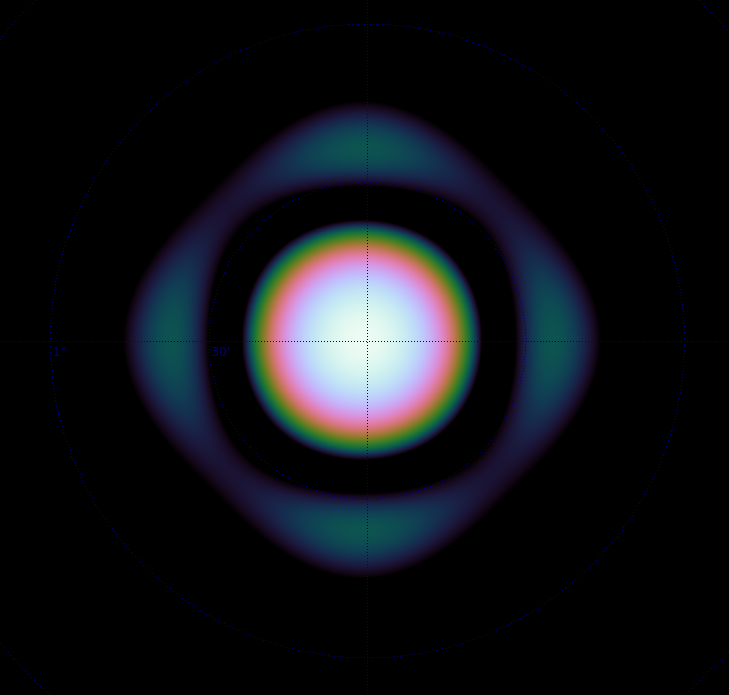
\includegraphics[scale=0.28]{Images/beam.png}
	\caption{Primary Beam Focus Pattern(\cite{oleg})}
\end{figure}
%
\subsubsection{Methods}\label{ra:ssec:meth}
%
\subsubsection{Errors}\label{ra:ssec:err}
%
\subsubsection{Error Correction}\label{ra:ssec:ec}
%--------------------------------------------------------------------------------------